%!TEX root = ../final-report.tex
\chapter{Results}
\label{ch:results}

This chapter presents results for the four solvers. For each of the five initial conditions, the solvers will be compared for a few representative bathymetries. Reference results were obtained using the unbalanced solver from Section~\ref{sec:roe} on a very fine grid of 10,000 cells. At the end, the execution time of the different solvers is compared as well.

\section{Still Water}

\begin{figure}
  \centering
  \begin{subfigure}{\textwidth}
    %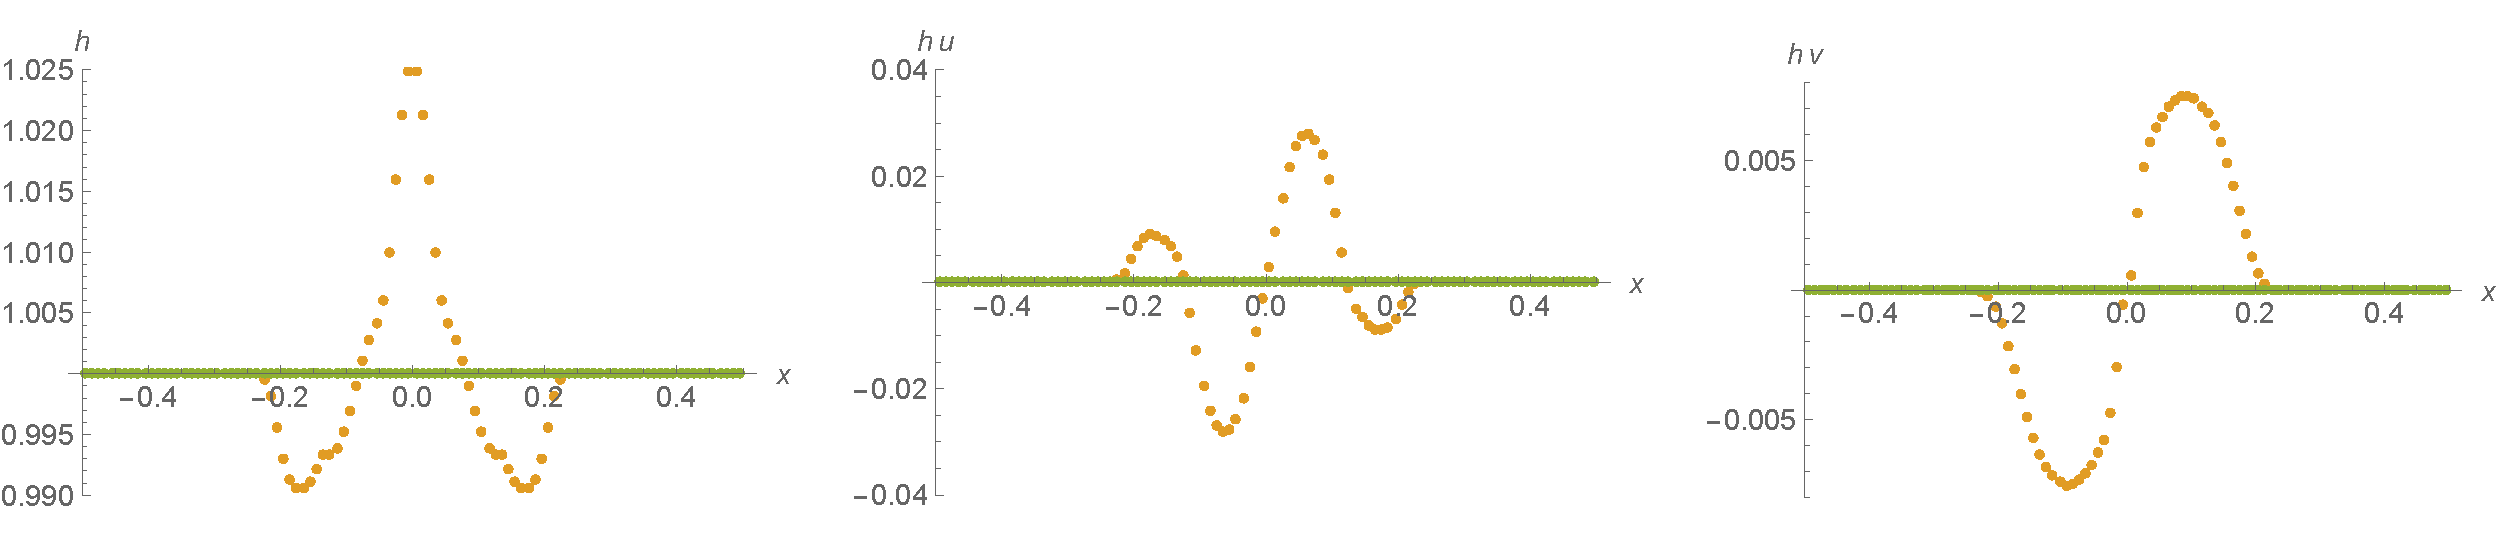
\includegraphics[width=\textwidth]{diagrams/results-still-1}
    \caption{$t = 0.1$}
    \label{fig:results-still-1}
  \end{subfigure} \\
  \begin{subfigure}{\textwidth}
    %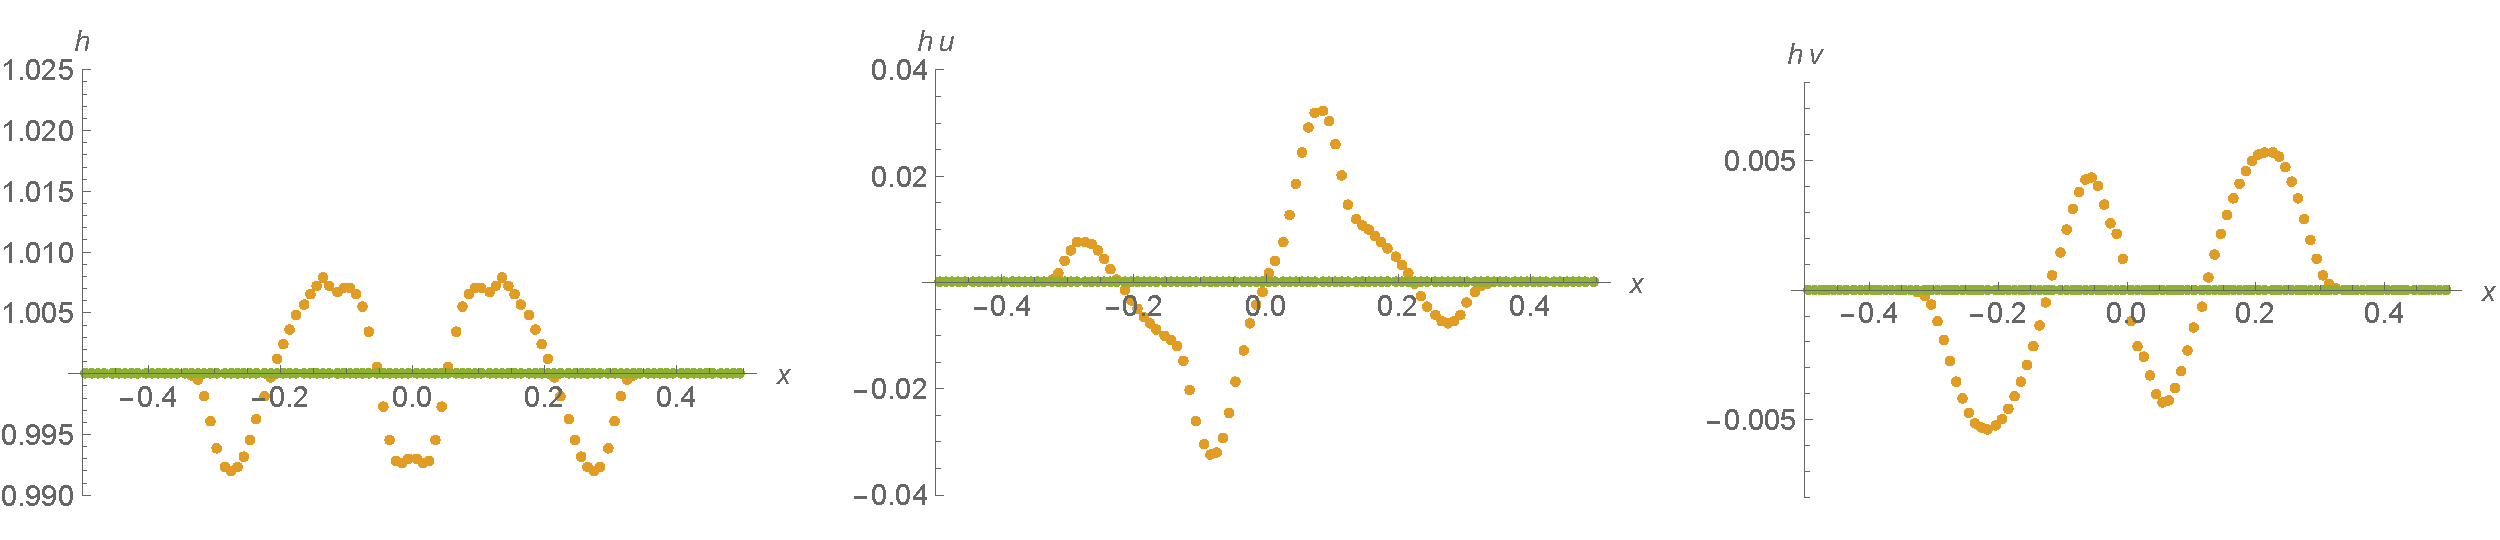
\includegraphics[width=\textwidth]{diagrams/results-still-2}
    \caption{$t = 0.2$}
    \label{fig:results-still-2}
  \end{subfigure} \\
  \begin{subfigure}{\textwidth}
    %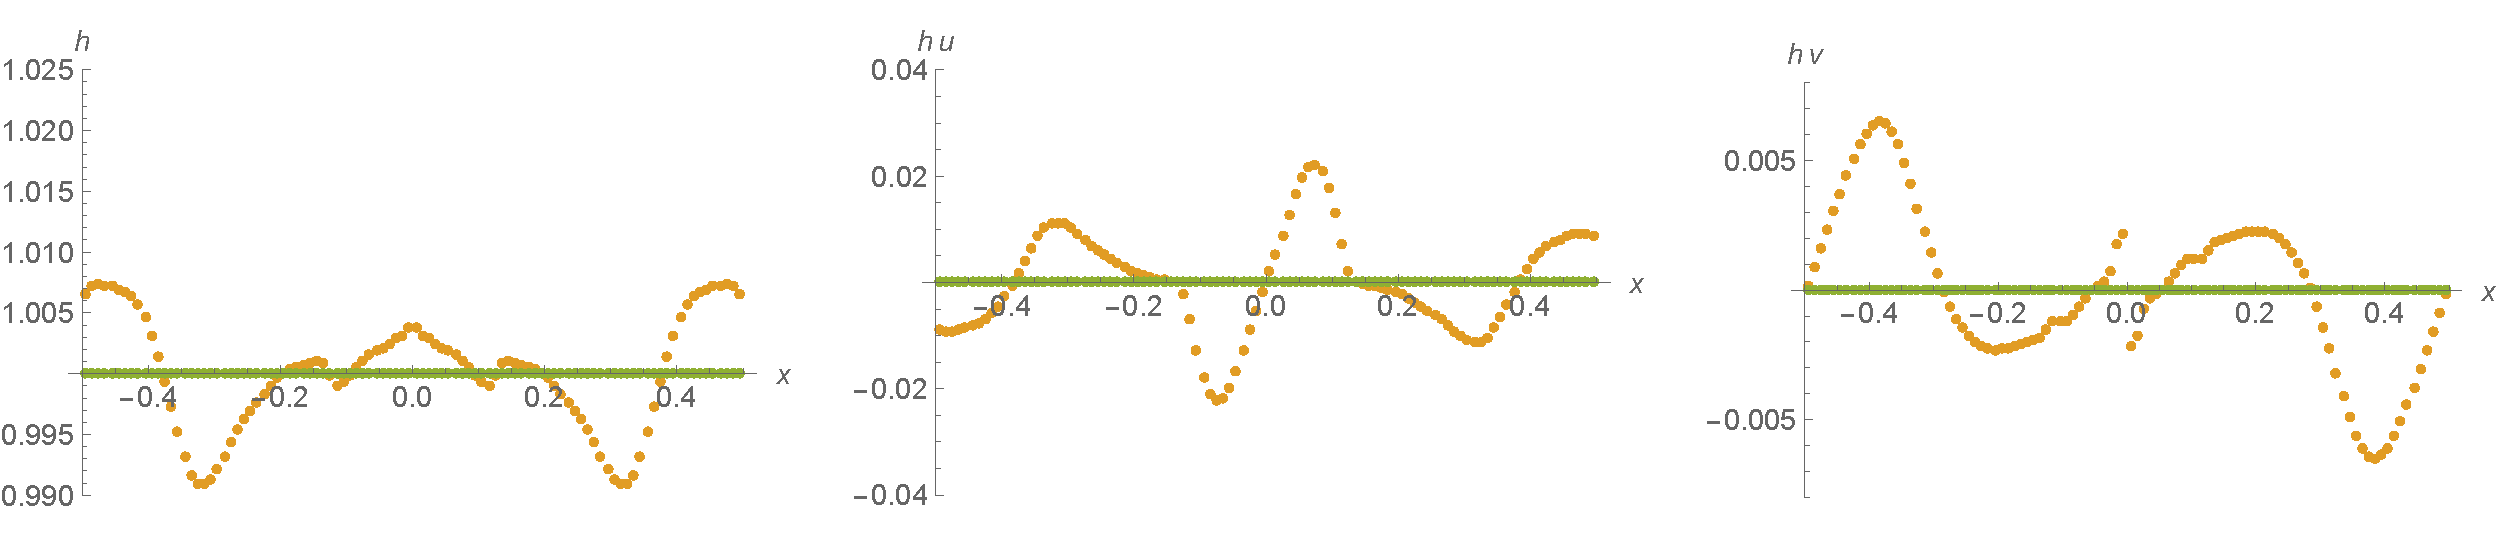
\includegraphics[width=\textwidth]{diagrams/results-still-5}
    \caption{$t = 0.5$}
    \label{fig:results-still-5}
  \end{subfigure} \\
  \begin{subfigure}{\textwidth}
    %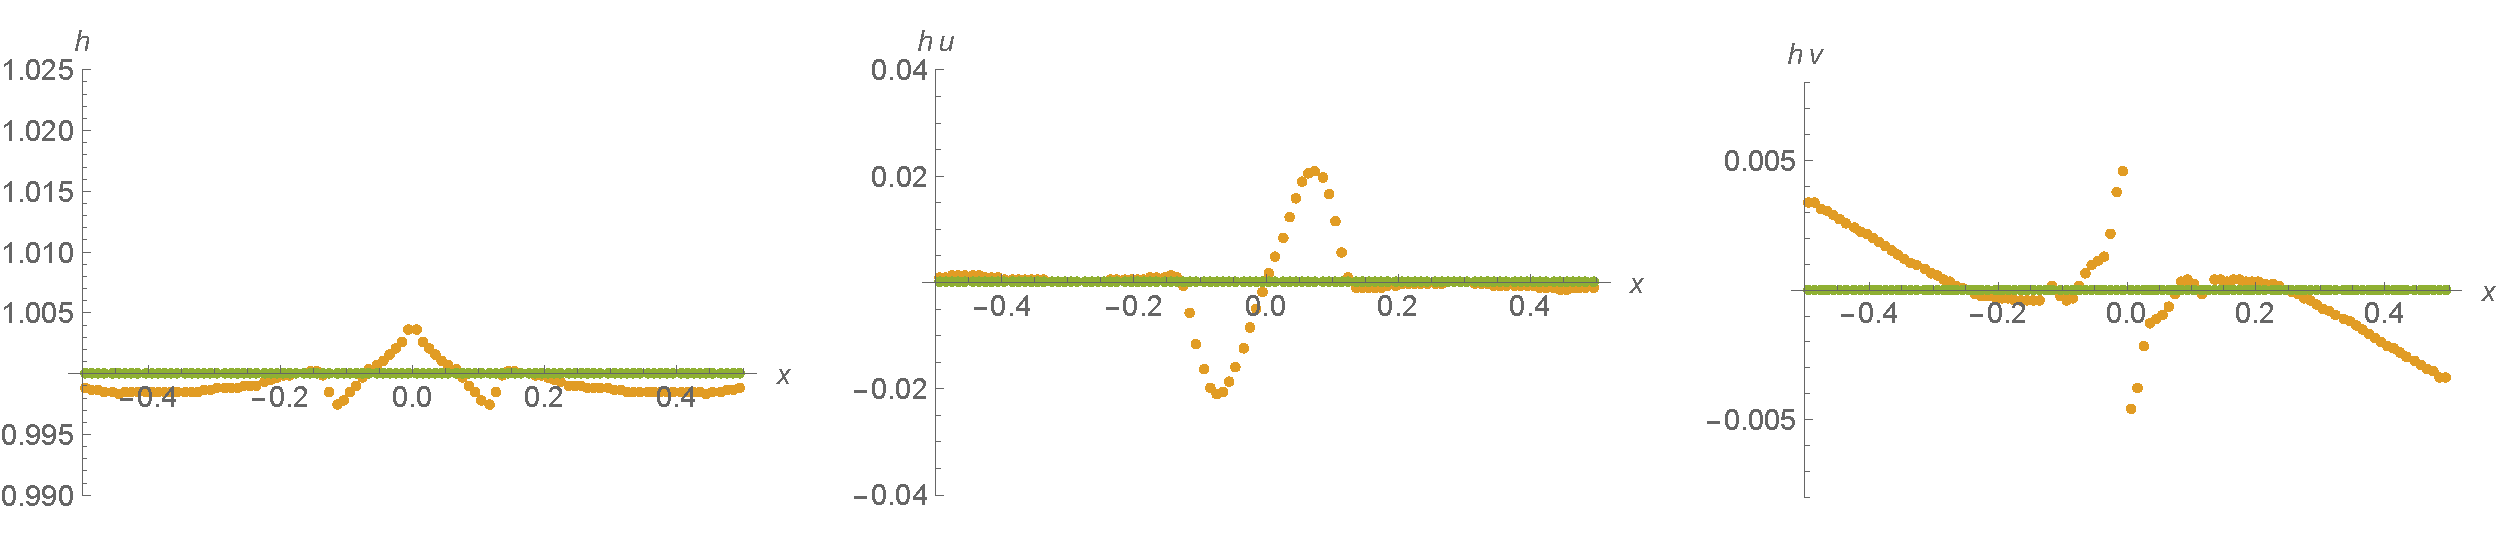
\includegraphics[width=\textwidth]{diagrams/results-still-10}
    \caption{$t = 1.0$}
    \label{fig:results-still-10}
  \end{subfigure}
  \caption{Results for still water over a cosine ridge. The exact solution is $h = 1$, $hu = hv = 0$ for all times. The orange data was obtained with the unbalanced solver over 100 grid cells. The green data corresponds to any of the three balanced solvers. The columns correspond to the conserved variables $h$, $hu$ and $hv$ and the rows to different time levels. $K = 10$.}
  \label{fig:results-still}
\end{figure}

The first system is simply still water over a cosine ridge, as shown in Fig.~\ref{fig:bath-cosine}. Figs~\ref{fig:results-still} show the results at times $t \in \{0.1, 0.2, 0.5, 1.0\}$. Only one set of data has been included for the three balanced solvers, as they are indistinguishable in the plot. All sets of data have been obtained for 100 grid cells and with $K = 10$.

Of course, these plots show exactly the motivation for developing balanced solvers in the first place: the unbalanced solver develops quite substantial waves, about 1\% of the water depth, and settles into a state which is not still with errors of about 0.5\%. From inspection across different grid sizes it appears that the size of the waves is proportional to $1/N$, whereas the error in the settled state is proportional to $1/N^2$.

It should be noted that the data for the two rogers solvers is exactly zero (since all terms that appear anywhere in the method are always zero), whereas the LeVeque solver is only zero to machine precision (since it relies on two separate computations to make the Riemann problems at the cell edges disappear).

\section{Wave through Still Water}

\begin{figure}
  \centering
  \begin{subfigure}{\textwidth}
    %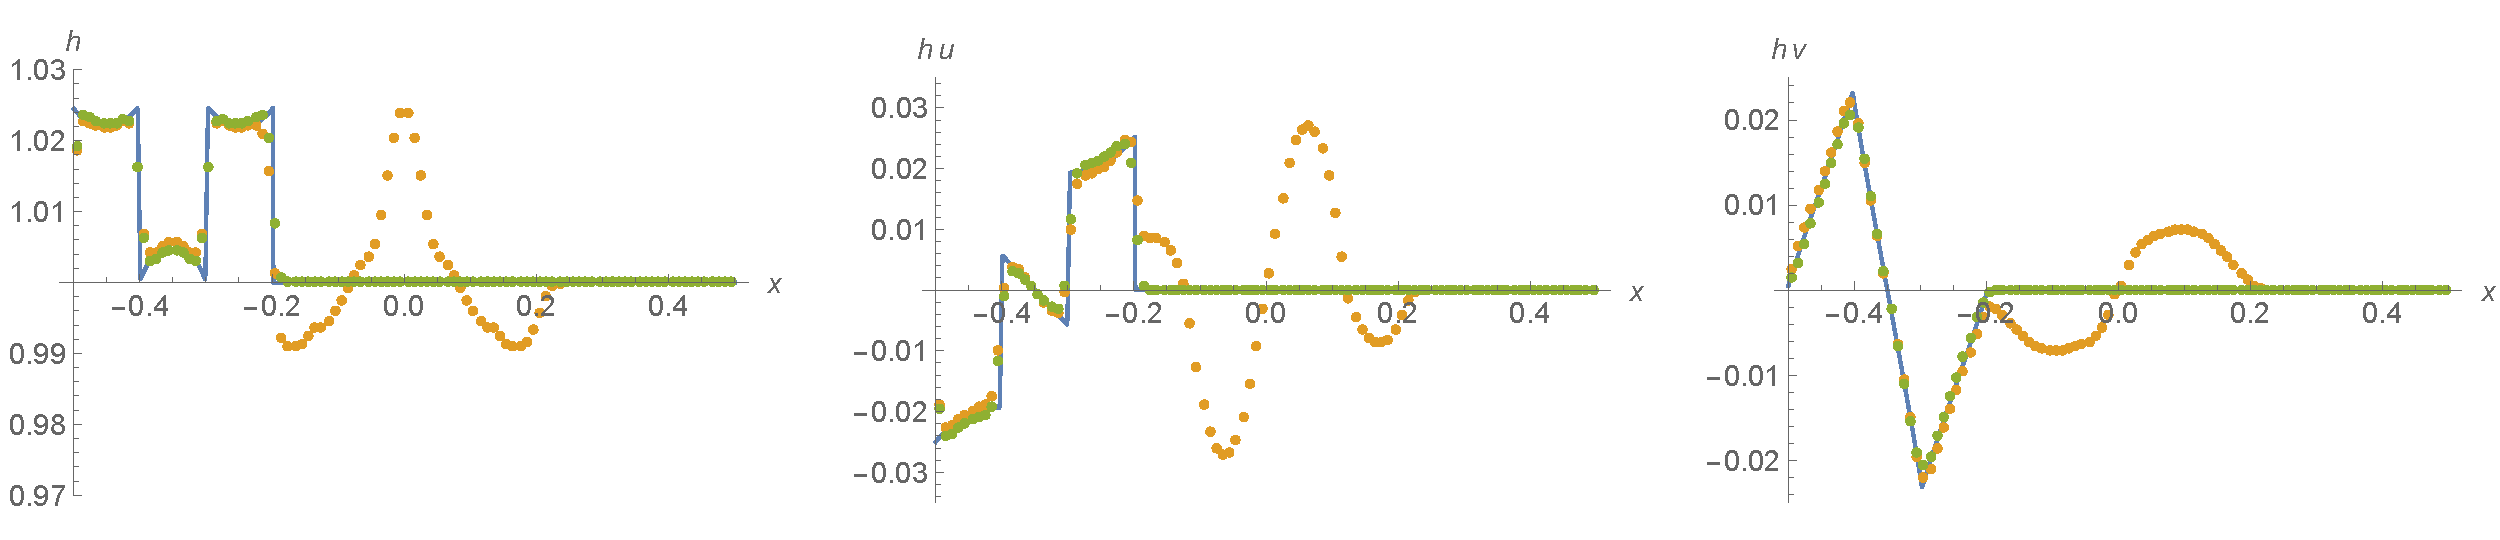
\includegraphics[width=\textwidth]{diagrams/results-wave-lev-1}
    \caption{$t = 0.1$}
    \label{fig:results-wave-lev-1}
  \end{subfigure} \\
  \begin{subfigure}{\textwidth}
    %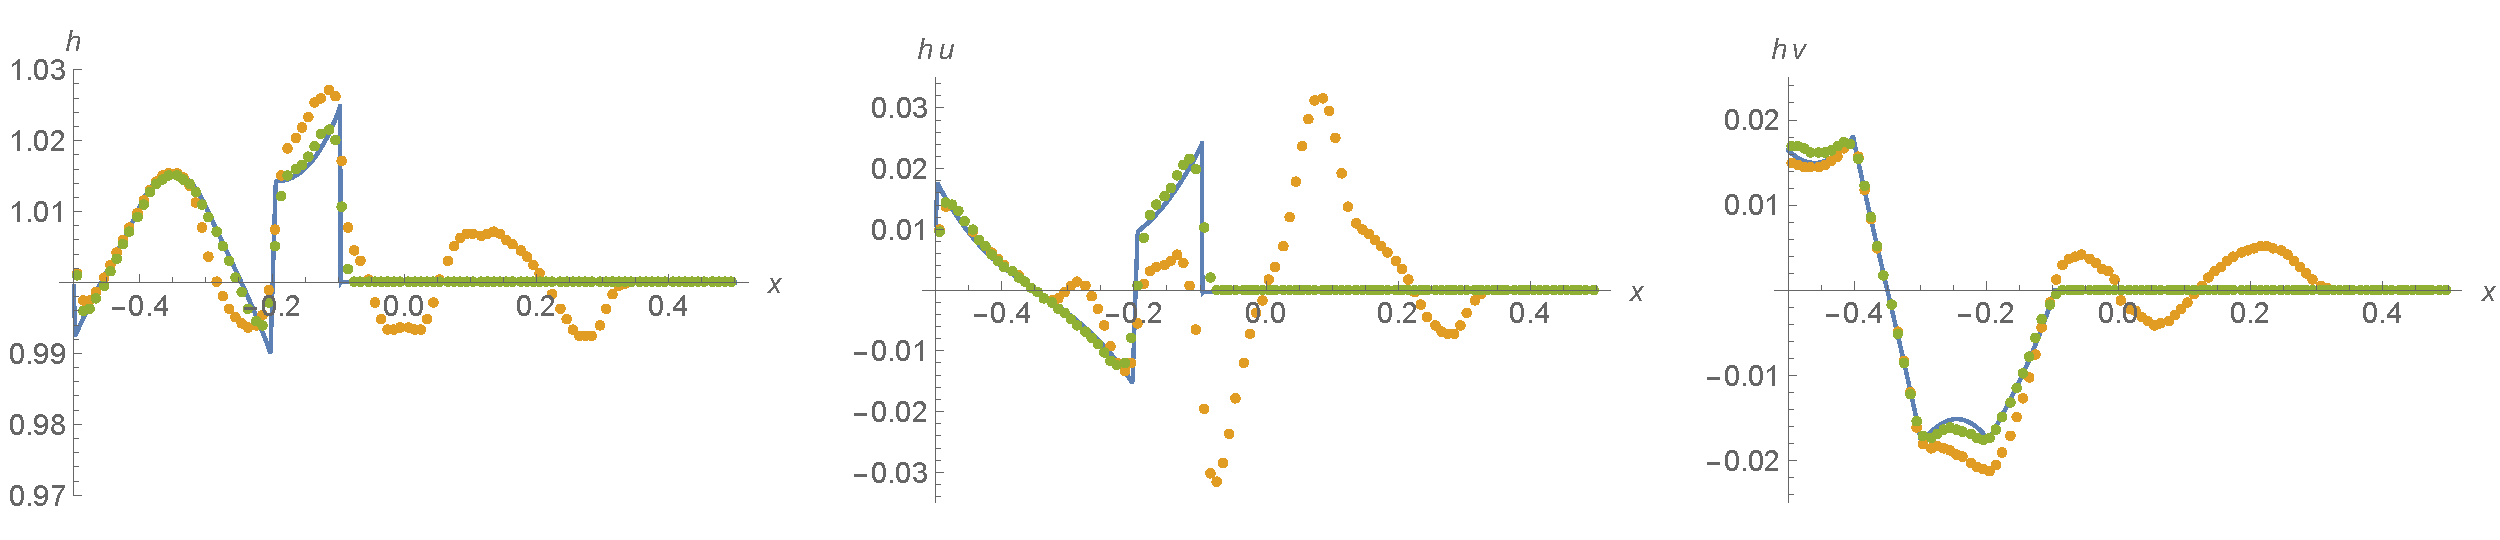
\includegraphics[width=\textwidth]{diagrams/results-wave-lev-2}
    \caption{$t = 0.2$}
    \label{fig:results-wave-lev-2}
  \end{subfigure} \\
  \begin{subfigure}{\textwidth}
    %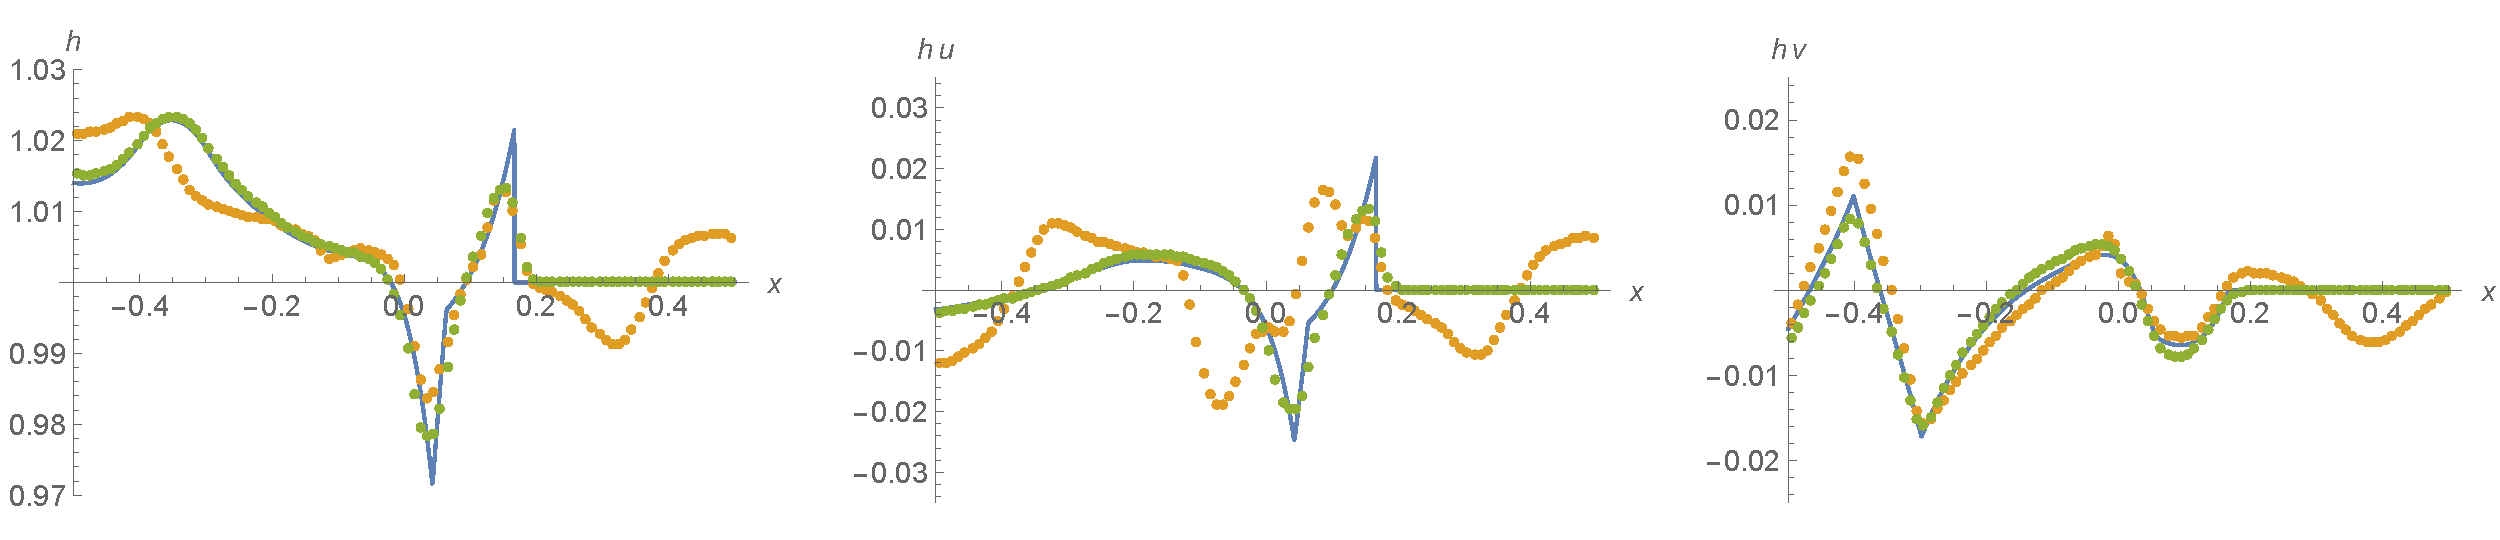
\includegraphics[width=\textwidth]{diagrams/results-wave-lev-5}
    \caption{$t = 0.5$}
    \label{fig:results-wave-lev-5}
  \end{subfigure} \\
  \begin{subfigure}{\textwidth}
    %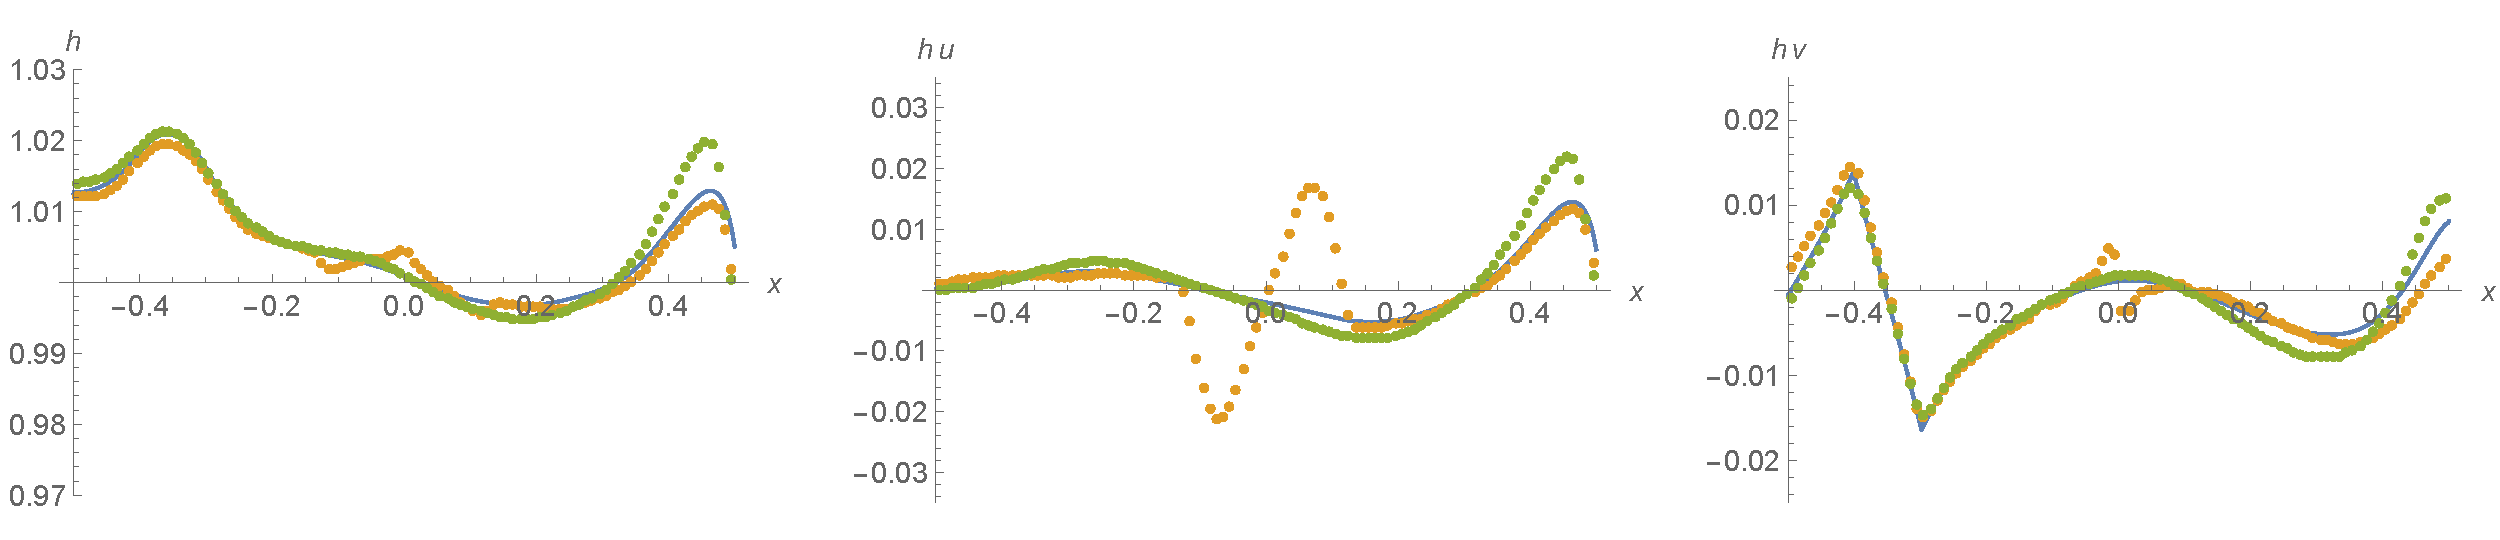
\includegraphics[width=\textwidth]{diagrams/results-wave-lev-10}
    \caption{$t = 1.0$}
    \label{fig:results-wave-lev-10}
  \end{subfigure}
  \caption{Results for wave through still water over a cosine ridge. The reference solution has been computed with the unbalanced solver on 10000 grid cells and is shown as a solid blue line. The orange data was obtained with the unbalanced solver over 100 grid cells. The green data corresponds to the LeVeque solver. The columns correspond to the conserved variables $h$, $hu$ and $hv$ and the rows to different time levels. $K = 10$.}
  \label{fig:results-wave-lev}
\end{figure}

\begin{figure}
  \centering
  \begin{subfigure}{\textwidth}
    %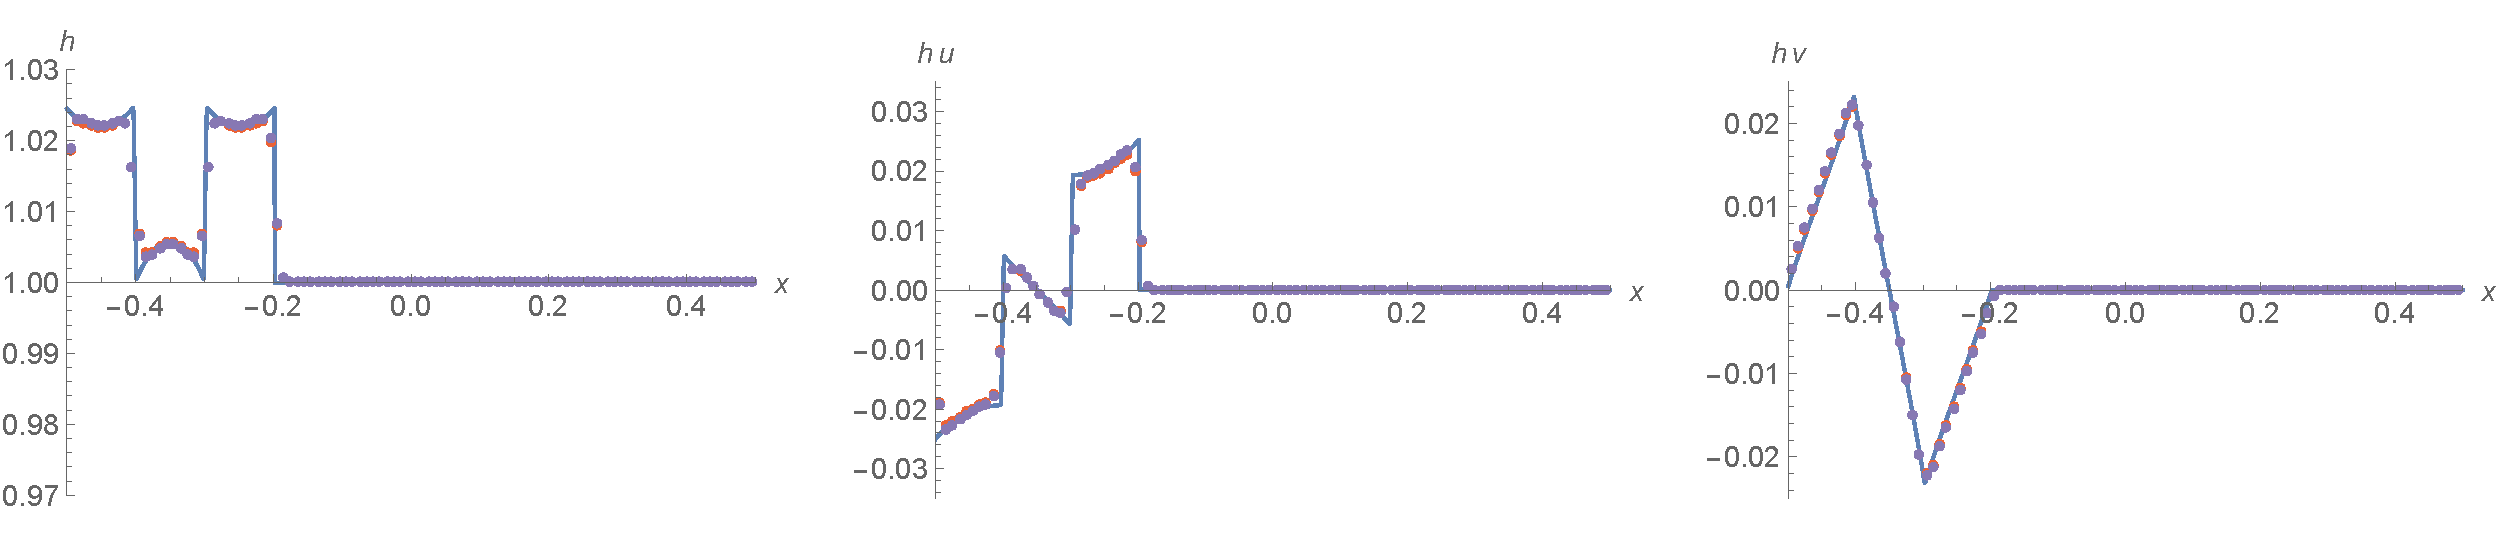
\includegraphics[width=\textwidth]{diagrams/results-wave-rog-1}
    \caption{$t = 0.1$}
    \label{fig:results-wave-rog-1}
  \end{subfigure} \\
  \begin{subfigure}{\textwidth}
    %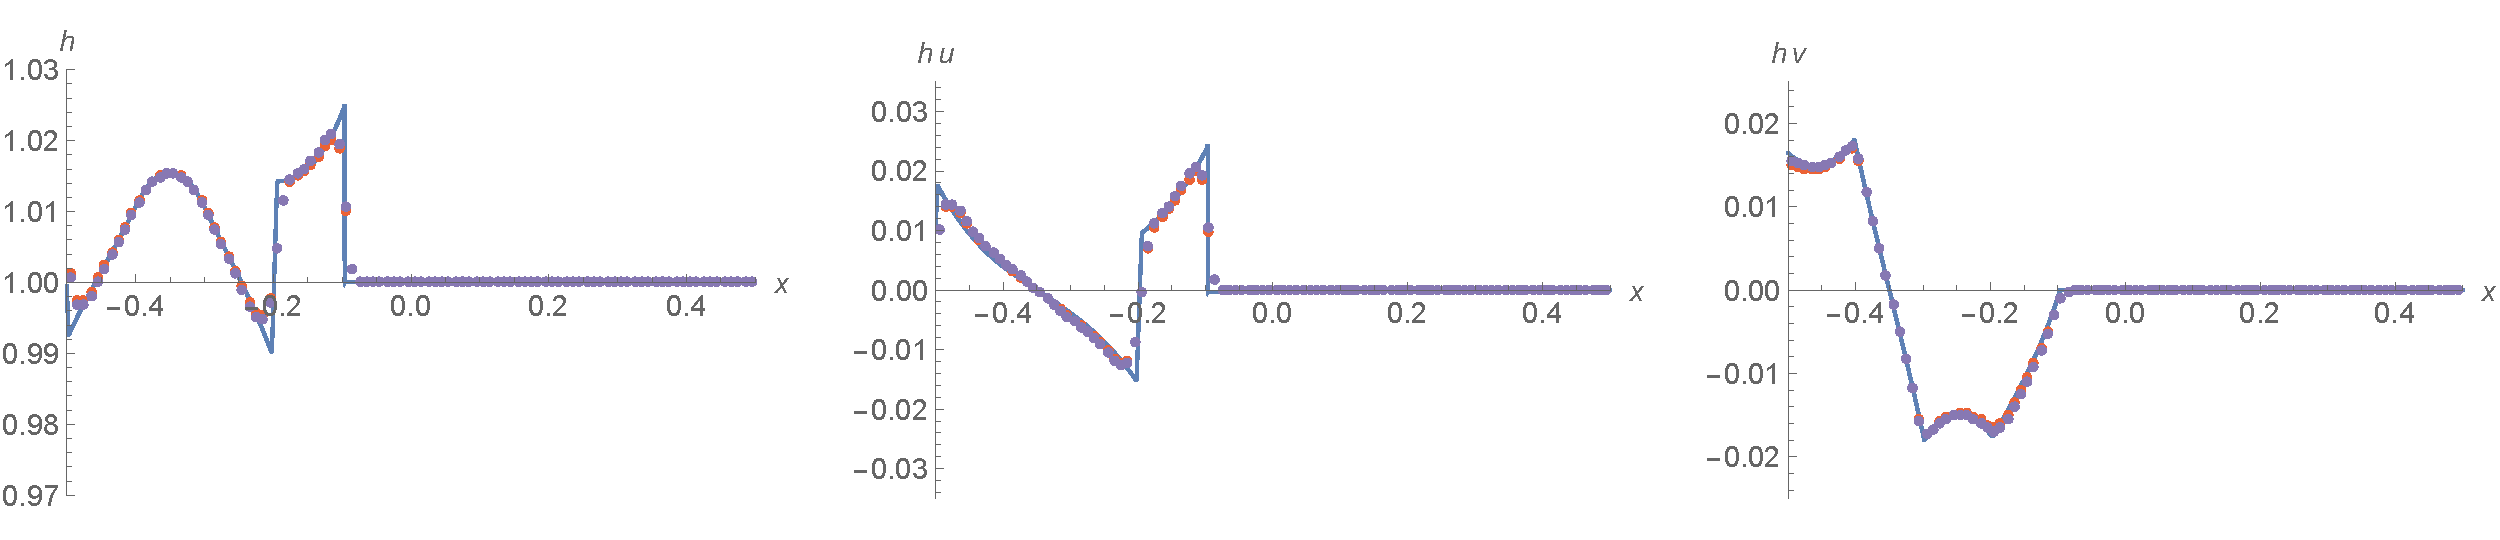
\includegraphics[width=\textwidth]{diagrams/results-wave-rog-2}
    \caption{$t = 0.2$}
    \label{fig:results-wave-rog-2}
  \end{subfigure} \\
  \begin{subfigure}{\textwidth}
    %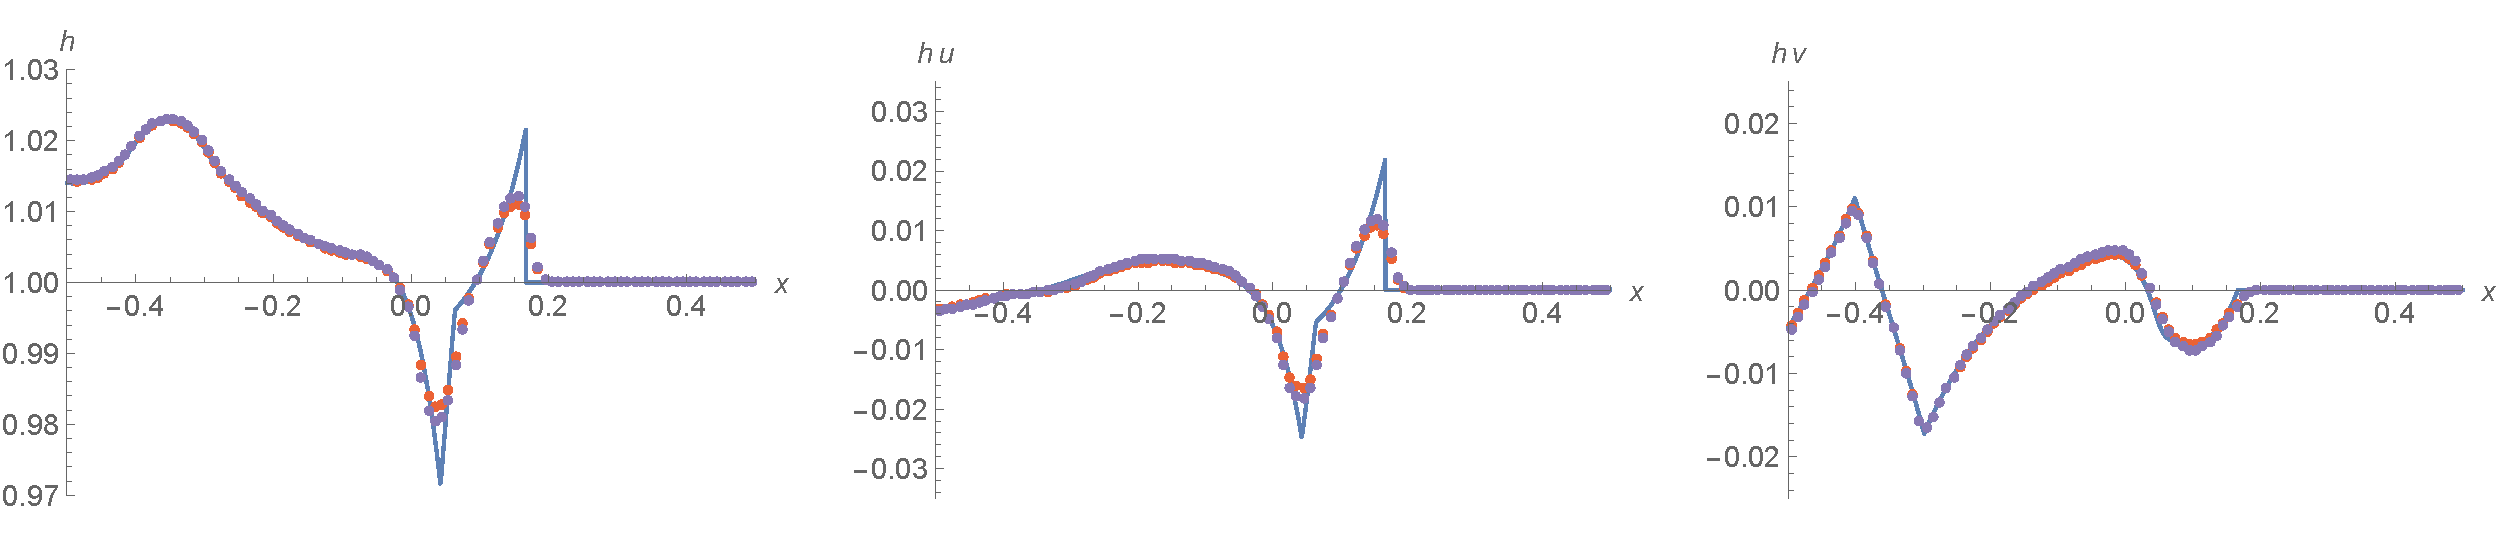
\includegraphics[width=\textwidth]{diagrams/results-wave-rog-5}
    \caption{$t = 0.5$}
    \label{fig:results-wave-rog-5}
  \end{subfigure} \\
  \begin{subfigure}{\textwidth}
    %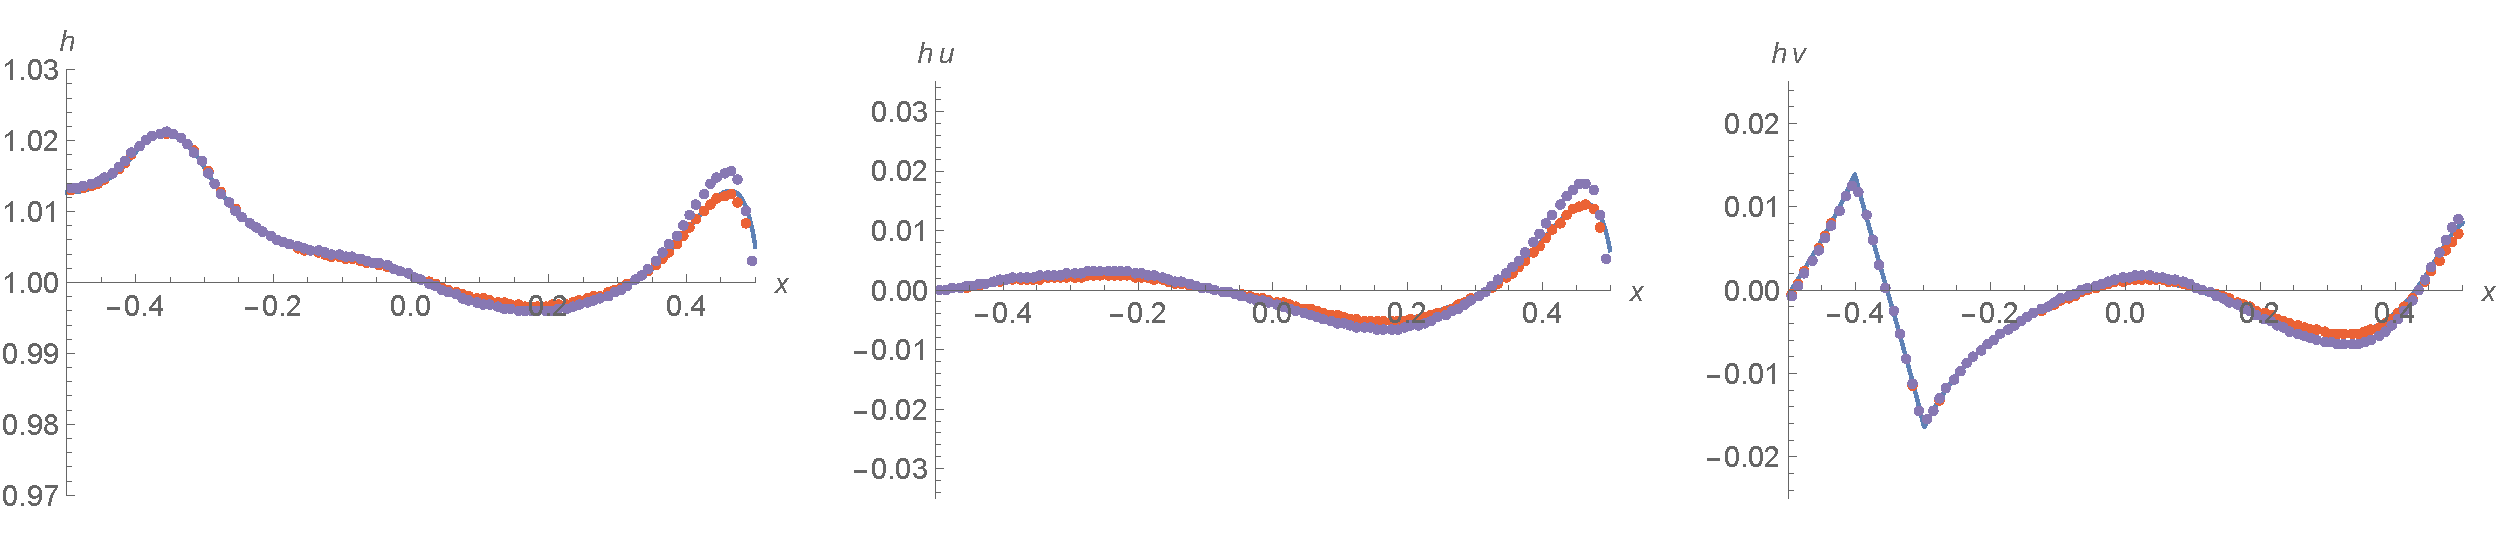
\includegraphics[width=\textwidth]{diagrams/results-wave-rog-10}
    \caption{$t = 1.0$}
    \label{fig:results-wave-rog-10}
  \end{subfigure}
  \caption{Results for wave through still water over a cosine ridge. The reference solution has been computed with the unbalanced solver on 10000 grid cells and is shown as a solid blue line. The red data was obtained with the Rogers solver for still water systems over 100 grid cells. The blue data corresponds to the Rogers solver for geostrophic equilibria. The columns correspond to the conserved variables $h$, $hu$ and $hv$ and the rows to different time levels. $K = 10$.}
  \label{fig:results-wave-rog}
\end{figure}

For this system a small perturbation is added to the surface profile of the water, near the left edge of the domain. The results for the unbalanced and LeVeque solver are shown in Figs.~\ref{fig:results-wave-lev}, those for Rogers solvers in Figs.~\ref{fig:results-wave-rog}.

It is notable that the unphysical waves of the balanced solver are comparable to the size of the real waves at this resolution, which makes the results very unreliable.

The balanced solver are much better at approximating the real solution, and produce very good results, considering the low resolution. It is hard to compare the performance of the three balanced solvers in detail, but it seems that the LeVeque solver produces the least accurate result, whereas the Rogers solver for still water systems approximates the real solution most closely.

\section{Geostrophic Equilibrium}

\begin{figure}
  \centering
  \begin{subfigure}{\textwidth}
    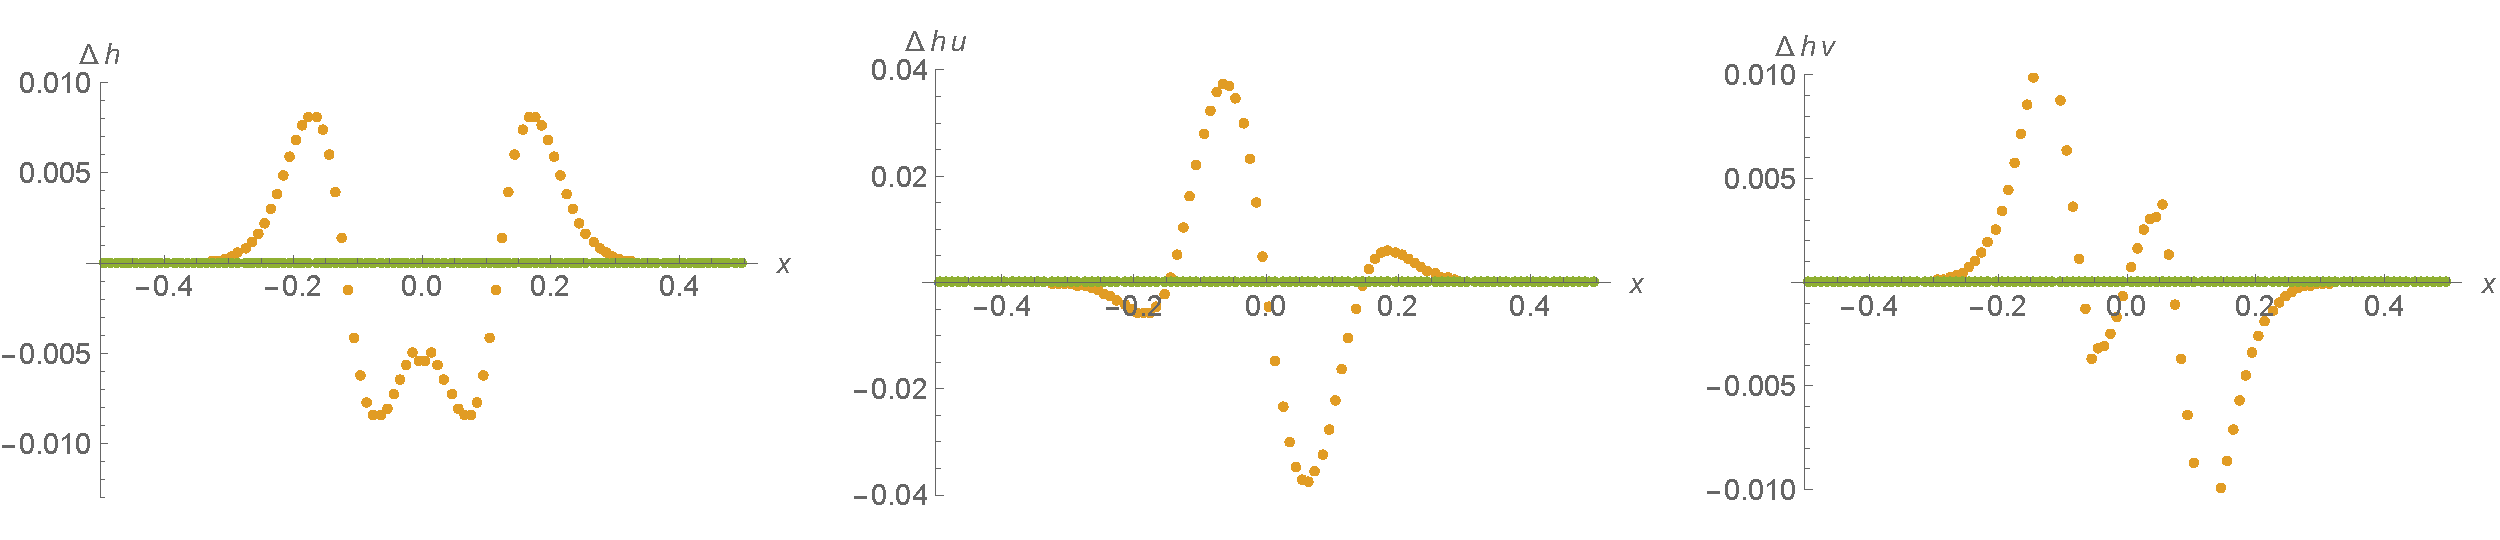
\includegraphics[width=\textwidth]{diagrams/results-geo-1}
    \caption{$t = 0.1$}
    \label{fig:results-geo-1}
  \end{subfigure} \\
  \begin{subfigure}{\textwidth}
    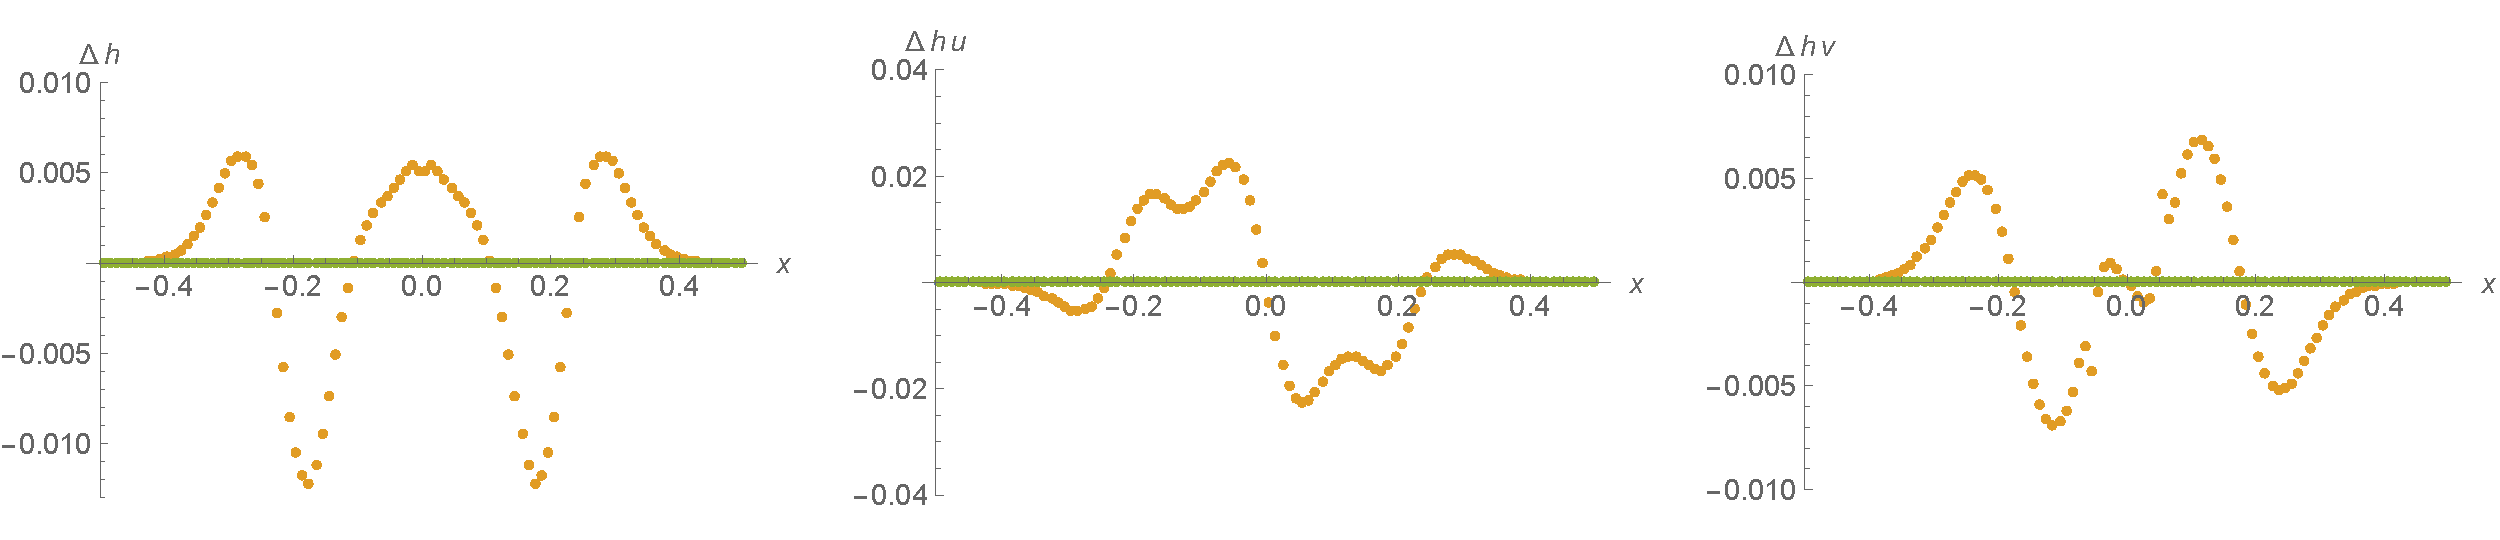
\includegraphics[width=\textwidth]{diagrams/results-geo-2}
    \caption{$t = 0.2$}
    \label{fig:results-geo-2}
  \end{subfigure} \\
  \begin{subfigure}{\textwidth}
    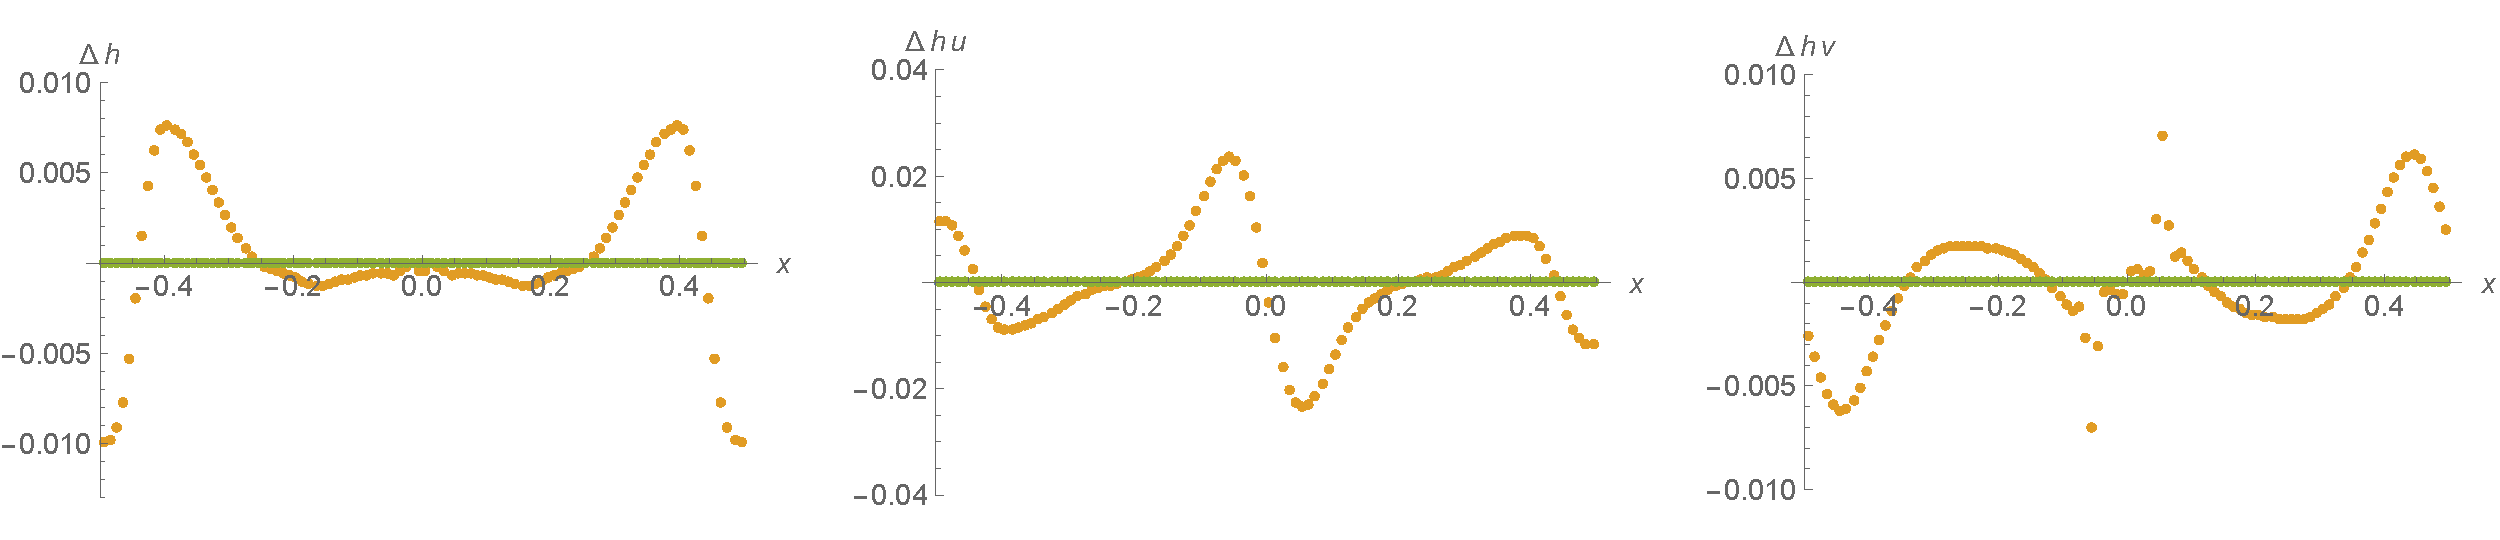
\includegraphics[width=\textwidth]{diagrams/results-geo-5}
    \caption{$t = 0.5$}
    \label{fig:results-geo-5}
  \end{subfigure} \\
  \begin{subfigure}{\textwidth}
    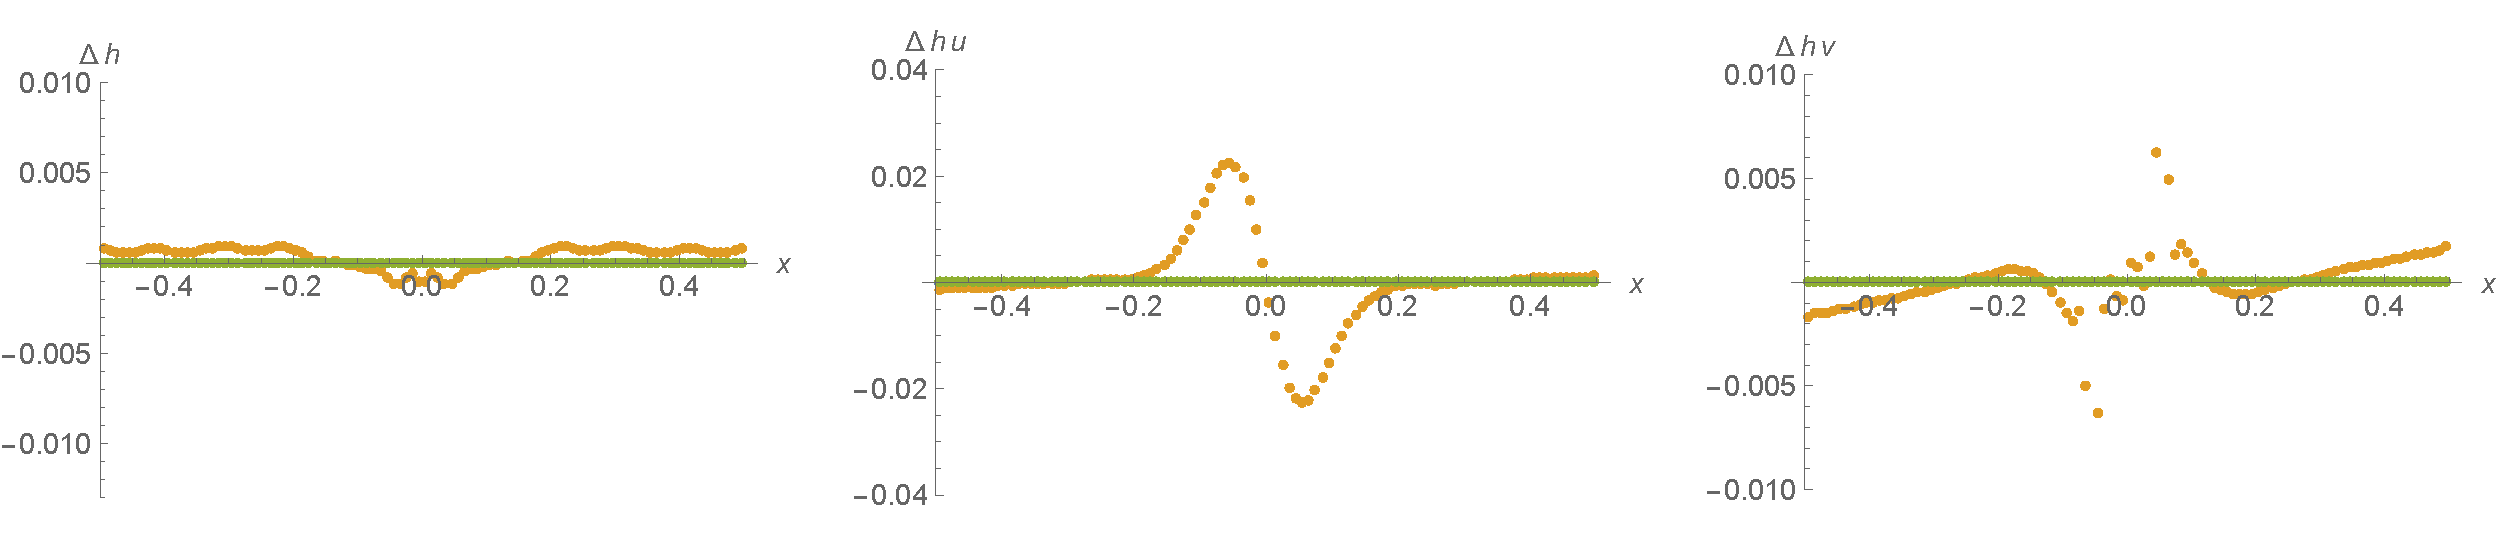
\includegraphics[width=\textwidth]{diagrams/results-geo-10}
    \caption{$t = 1.0$}
    \label{fig:results-geo-10}
  \end{subfigure}
  \caption{Results for geostrophic equilibrium. The equilibrium state has been subtracted off the plots, such that the exact solution is $\Delta h = \Delta hu = \Delta hv = 0$. The orange data corresponds to both the unbalanced solver and the Rogers solver for still water over 100 grid cells. The green data corresponds to both the LeVeque solver and the Rogers solver for geostrophic equilibria. The columns correspond to the conserved variables $h$, $hu$ and $hv$ and the rows to different time levels. $K = 10$.}
  \label{fig:results-geo}
\end{figure}

The results for geostrophic equilibrium (with Gaussian surface profile) over flat bathymetry is shown in Figs.~\ref{fig:results-geo}. As opposed to the previous two systems, these plots show only deviations from the equilibrium state, since errors would be barely visible otherwise.

The unbalanced solver and the Rogers solver for still water systems give identical results. This was to be expected, as the Coriolis term is unchanged for this solver. The magnitude of the generated waves is comparable to the still water case. This is also not surprising, as the gradients of $h$ are on the same order for both setups.

Both the LeVeque solver and the Rogers solver for geostrophic equilibria preserve the state exactly, as desired. Note that, as in the still water case, only for the Rogers solver are the deviations exactly zero. The LeVeque solver preserves the equilibrium to machine precision.

\section{Wave through Geostrophic Equilibrium}

\section{Uniform Flow}

\section{Execution Time}

\begin{itemize}
  \item show how unbalanced method fails
  \item go through different methods, showing where they work and where they fail
\end{itemize}